\documentclass{article}

\usepackage{amsmath} % for mathmatical notation
\usepackage{graphicx}
\usepackage{listings}
\usepackage{color}
\title{My first document}
\date{October, 19, 2015}
\author{Andrew Heng}



\renewcommand\lstlistingname{Quelltext} % Change language of section name

\lstset{ % General setup for the package
	language=Python,
	basicstyle=\small\sffamily,
	%basicstyle=\ttfamily\footnotesize,
	%numbers=left,
 	%numberstyle=\tiny,
	%frame=tb,
	tabsize=4,
	%columns=fixed,
	%showstringspaces=false,
	%showtabs=false,
	%keepspaces
}
\begin{document}
	\pagenumbering{gobble} % turn off page number
	\maketitle
	\newpage
	\pagenumbering{arabic} % turn page number on

\tableofcontents
\newpage

\section{Section} %font w/ number	
Hello World!
\subsection{Subsection} %smaller version of a subsection
Structuring a document is easy!
\subsubsection{subsubsection}
More text.
\paragraph{Paragraph}
Some paragraph text
\section{Another Section}
my favourite equation\\
\begin{equation*}
f(x) = x^2
\end{equation*}

\begin{align} % & and align will make nice steps
y &= \frac{1}{(x-2)^2}\\
y &= \frac{1}{x^2-4x+4}\\
\end{align}

Volume of a disc
\begin{equation}
V = \int^a_b  \pi r^2
\end{equation}


\newpage
\section{Graph}
\begin{figure}
	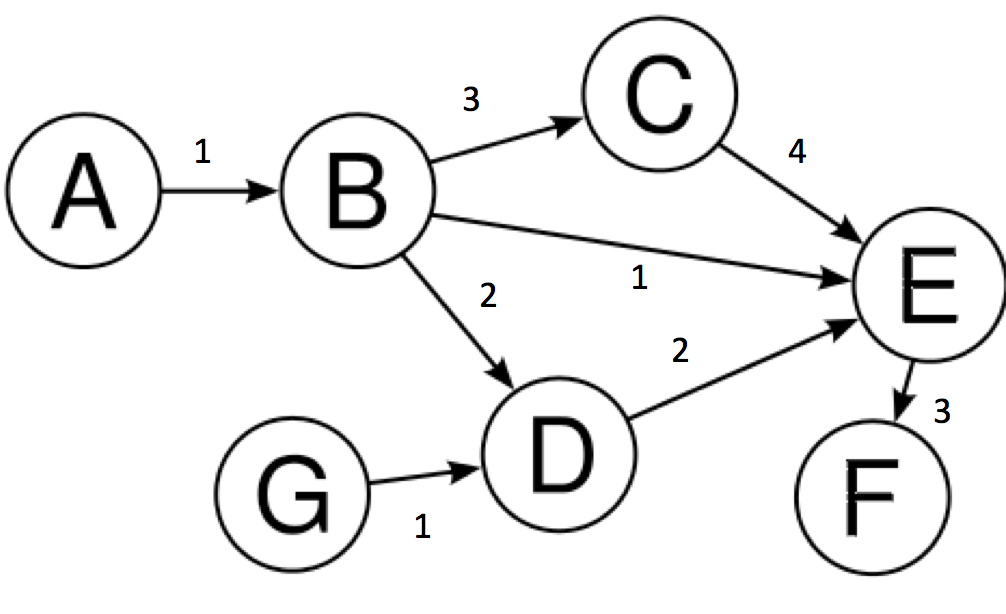
\includegraphics[width=\linewidth]{graph.png} %width =\linewidth to fit image on page
	\caption{Dijktra algorithm}
	\label{fig:graph}
\end{figure}

Figure \ref{fig:graph} shows a node A going to node F %refer back to the label

\begin{lstlisting}
def gcd(a, b):
	if(b==0):return a
	else:  return gcd(b, a%b)
\end{lstlisting}

\end{document}

